\subsection{Sensor}
I dette afsnit diskuteres forskellige sensorer, deres specifikationer og der dannes grundlag for valg af sensor. \newline

\subsubsection{Kriterier for valg af sensor:} 
\begin{enumerate}
	\item[•]Forbindelsetype		
	\item[•]Præcision på sensoren 
	\item[•]Måleafstand			
	\item[•]Driftsspænding
	\item[•]Pris
\end{enumerate} 

I forbindelse med kriterierne sat for valg af sensor samt kravene i kravspecifikationen er temperatur sensor DALLAS18B20 (DS18B20) valgt til måling af vandrør. Alle sensorer i tabel 3.1 er digitale, hvoraf kun DS18B20 kan monteres ved hjælp af THT(Through-Hole Technology) hvilket kan være en fordel under montering. 
 
\begin{table}[h]
\centering
\begin{tabular}{|l|l|l|l|l|}
\hline
\rowcolor{lightgray} & LM9523 & LM53DIMA & LM86CIM & DS18B20 \\ \hline
Præcision & $\pm$1 $^{\circ}$C, $\pm$2.5 $^{\circ}$C & $\pm$1 $^{\circ}$C, $\pm$3 $^{\circ}$C & $\pm$1 $^{\circ}$C, $\pm$3 $^{\circ}$C & \begin{tabular}[c]{@{}l@{}}$\pm$0,5 $^{\circ}$C (ved -10 \\ til +85 $^{\circ}$C)\end{tabular} \\ \hline
Driftstemperatur & 0 $^{\circ}$C til +85 $^{\circ}$C & 0 $^{\circ}$C til 85 $^{\circ}$C & 0 $^{\circ}$C til 85 $^{\circ}$C & -55 $^{\circ}$C til 125 $^{\circ}$C \\ \hline
Montering & SMD & SMD & SMD & THT \\ \hline
Pris & 18,10 DKK & 18,85 DKK & 11,864 DKK & 35,20 DKK \\ \hline
Driftsspænding & 3,0 V til 3,6 V & 3,0 V til 3,6 V & 3,0 V til 3,6 V & 3,0 V til 5,5V \\ \hline
\end{tabular}
\caption{Tabel over mulige valg af sensorer}
\label{sensor_tabel}
\end{table}
\newpage
  

DS18B20, i kontrast til de resterende vist i tabel 3.1, besidder den mest nøjagtige præcision samt opfylder kravene i kravspecifikationen med en driftstemperatur på 0-100 $^{\circ}$C. Ds18B20 er en digital temperatur sensor som foretager målinger med en opløsning på 9-12 bit. 
\newline
\newline
Sensoren kommunikerer via en 1-Wire bus forbindelse, som tillader op til flere sensorer på samme forbindelse. Denne forbindelse kræver kun en enkelt datalinie for at kommunikere med mikroprocessoren. Denne ene datalinie kan samtidig anvendes som strømforsyning til sensoren. Dette forstås som "parasite power".

\begin{figure}[h!]
  \centering
  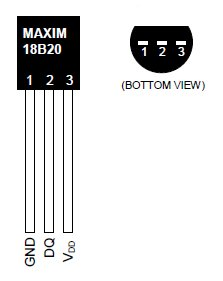
\includegraphics[width=0.3\textwidth]{figures/ds18b20-pinout.jpg}
  \caption{Tegning over DS18B20 temperatur sensor. Foto af: http://www.hobbytronics.co.uk}
  \label{ds18b20_pins}
\end{figure} 

Til målingen af rumtemperaturen er sensoren DHT11 valgt. Denne er en digital sensor som måler både temperatur og ændringer i luftfugtigheden. Denne sensor kræver en strømtilførsel på 3,0-5,0 V. \newline
Sensoren kan måle temperaturændringer inden for 0-50 $^{\circ}$C med en præcision på $\pm$2 $^{\circ}$C, samt måle luftfugtighedsændringer inden for 20-80\% fugtighed med en præcision på 5\%. 
Denne sensor er valgt med forbehold i tilfælde af at temperaturen i rummet påvirkes af luftfugtigheden.

\begin{figure}[h!]
  \centering
  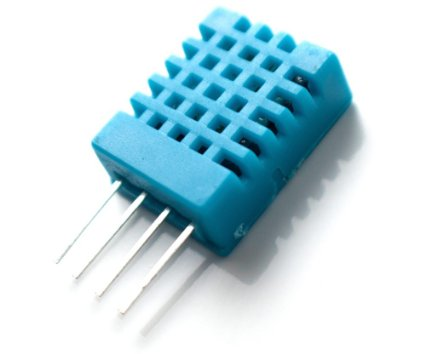
\includegraphics[width=0.3\textwidth]{figures/DHT11.jpg}
  \caption{DHT11 temperatur- og luftfugtighedssensor. Foto af: http://www.spikenzielabs.com}
  \label{dht11_billede}
\end{figure} 
   






\newpage
